\documentclass[11pt]{article}
%\usepackage[hyperref]{acl2017}
\usepackage[nohyperref]{acl2017}
\usepackage{times}
\usepackage{url}
\usepackage{latexsym}
\usepackage{booktabs}
\usepackage{multirow}
\usepackage{graphicx}  %%% for including graphics
\usepackage{rotating}
\usepackage{color}


%\aclfinalcopy % Uncomment this line for the final submission
\def\aclpaperid{489} %  Enter the acl Paper ID here

%\setlength\titlebox{5cm}
% You can expand the titlebox if you need extra space
% to show all the authors. Please do not make the titlebox
% smaller than 5cm (the original size); we will check this
% in the camera-ready version and ask you to change it back.

\newcommand\BibTeX{B{\sc ib}\TeX}

\newcommand{\sz}[1]{\textcolor{blue}{\emph{//sz: #1//}}}
\newcommand{\das}[1]{\textcolor{red}{\emph{//das: #1//}}}
\newcommand{\refexp}[1]{\textsl{#1}}
\newcommand{\word}[1]{\textsl{#1}}
\newcommand{\cat}[1]{\textsc{#1}}
\newcommand{\vgenome}{VisualGenome\xspace}



%\title{What do you need to know about a word when you\\ want to use it for naming objects?}
\title{How many times must an object be named (before we know what it is)?}


\author{Sina Zarrie{\ss}  \and David Schlangen\\
  Dialogue Systems Group // CITEC // Faculty of Linguistics and Literary Studies \\
 Bielefeld University, Germany \\
  {\tt \{sina.zarriess,david.schlangen\}@uni-bielefeld.de} \\}

\date{}



\begin{document}

\maketitle

\begin{abstract}
\end{abstract}


\section{Introduction}

The real-world objects that we interact with in our every-day life can be categorized into many thousands and maybe millions of categories. And even a single object can be member of many categories, i.e.\ at different taxonomical levels or in different parts of a taxonomy. For instance, both objects in Figure \ref{fig:cake} are at once instances of \cat{cake}, \cat{cheesecake}, \cat{dessert}, \cat{sweet}, \cat{pastry}, \cat{food} etc.

\begin{figure}[htbp]
\begin{center}
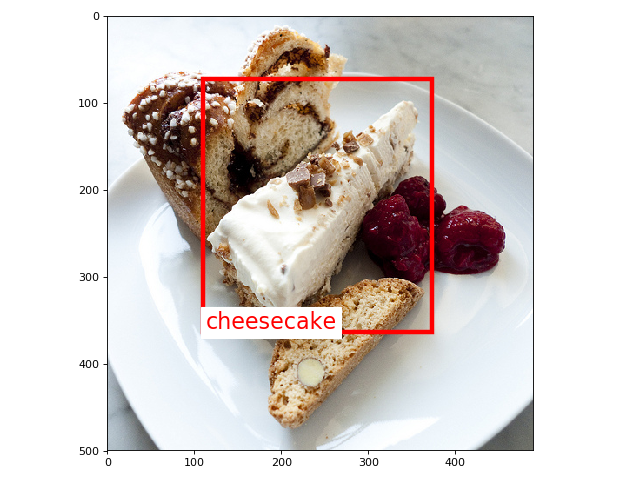
\includegraphics[height=3cm]{Figures/cheescake.png}
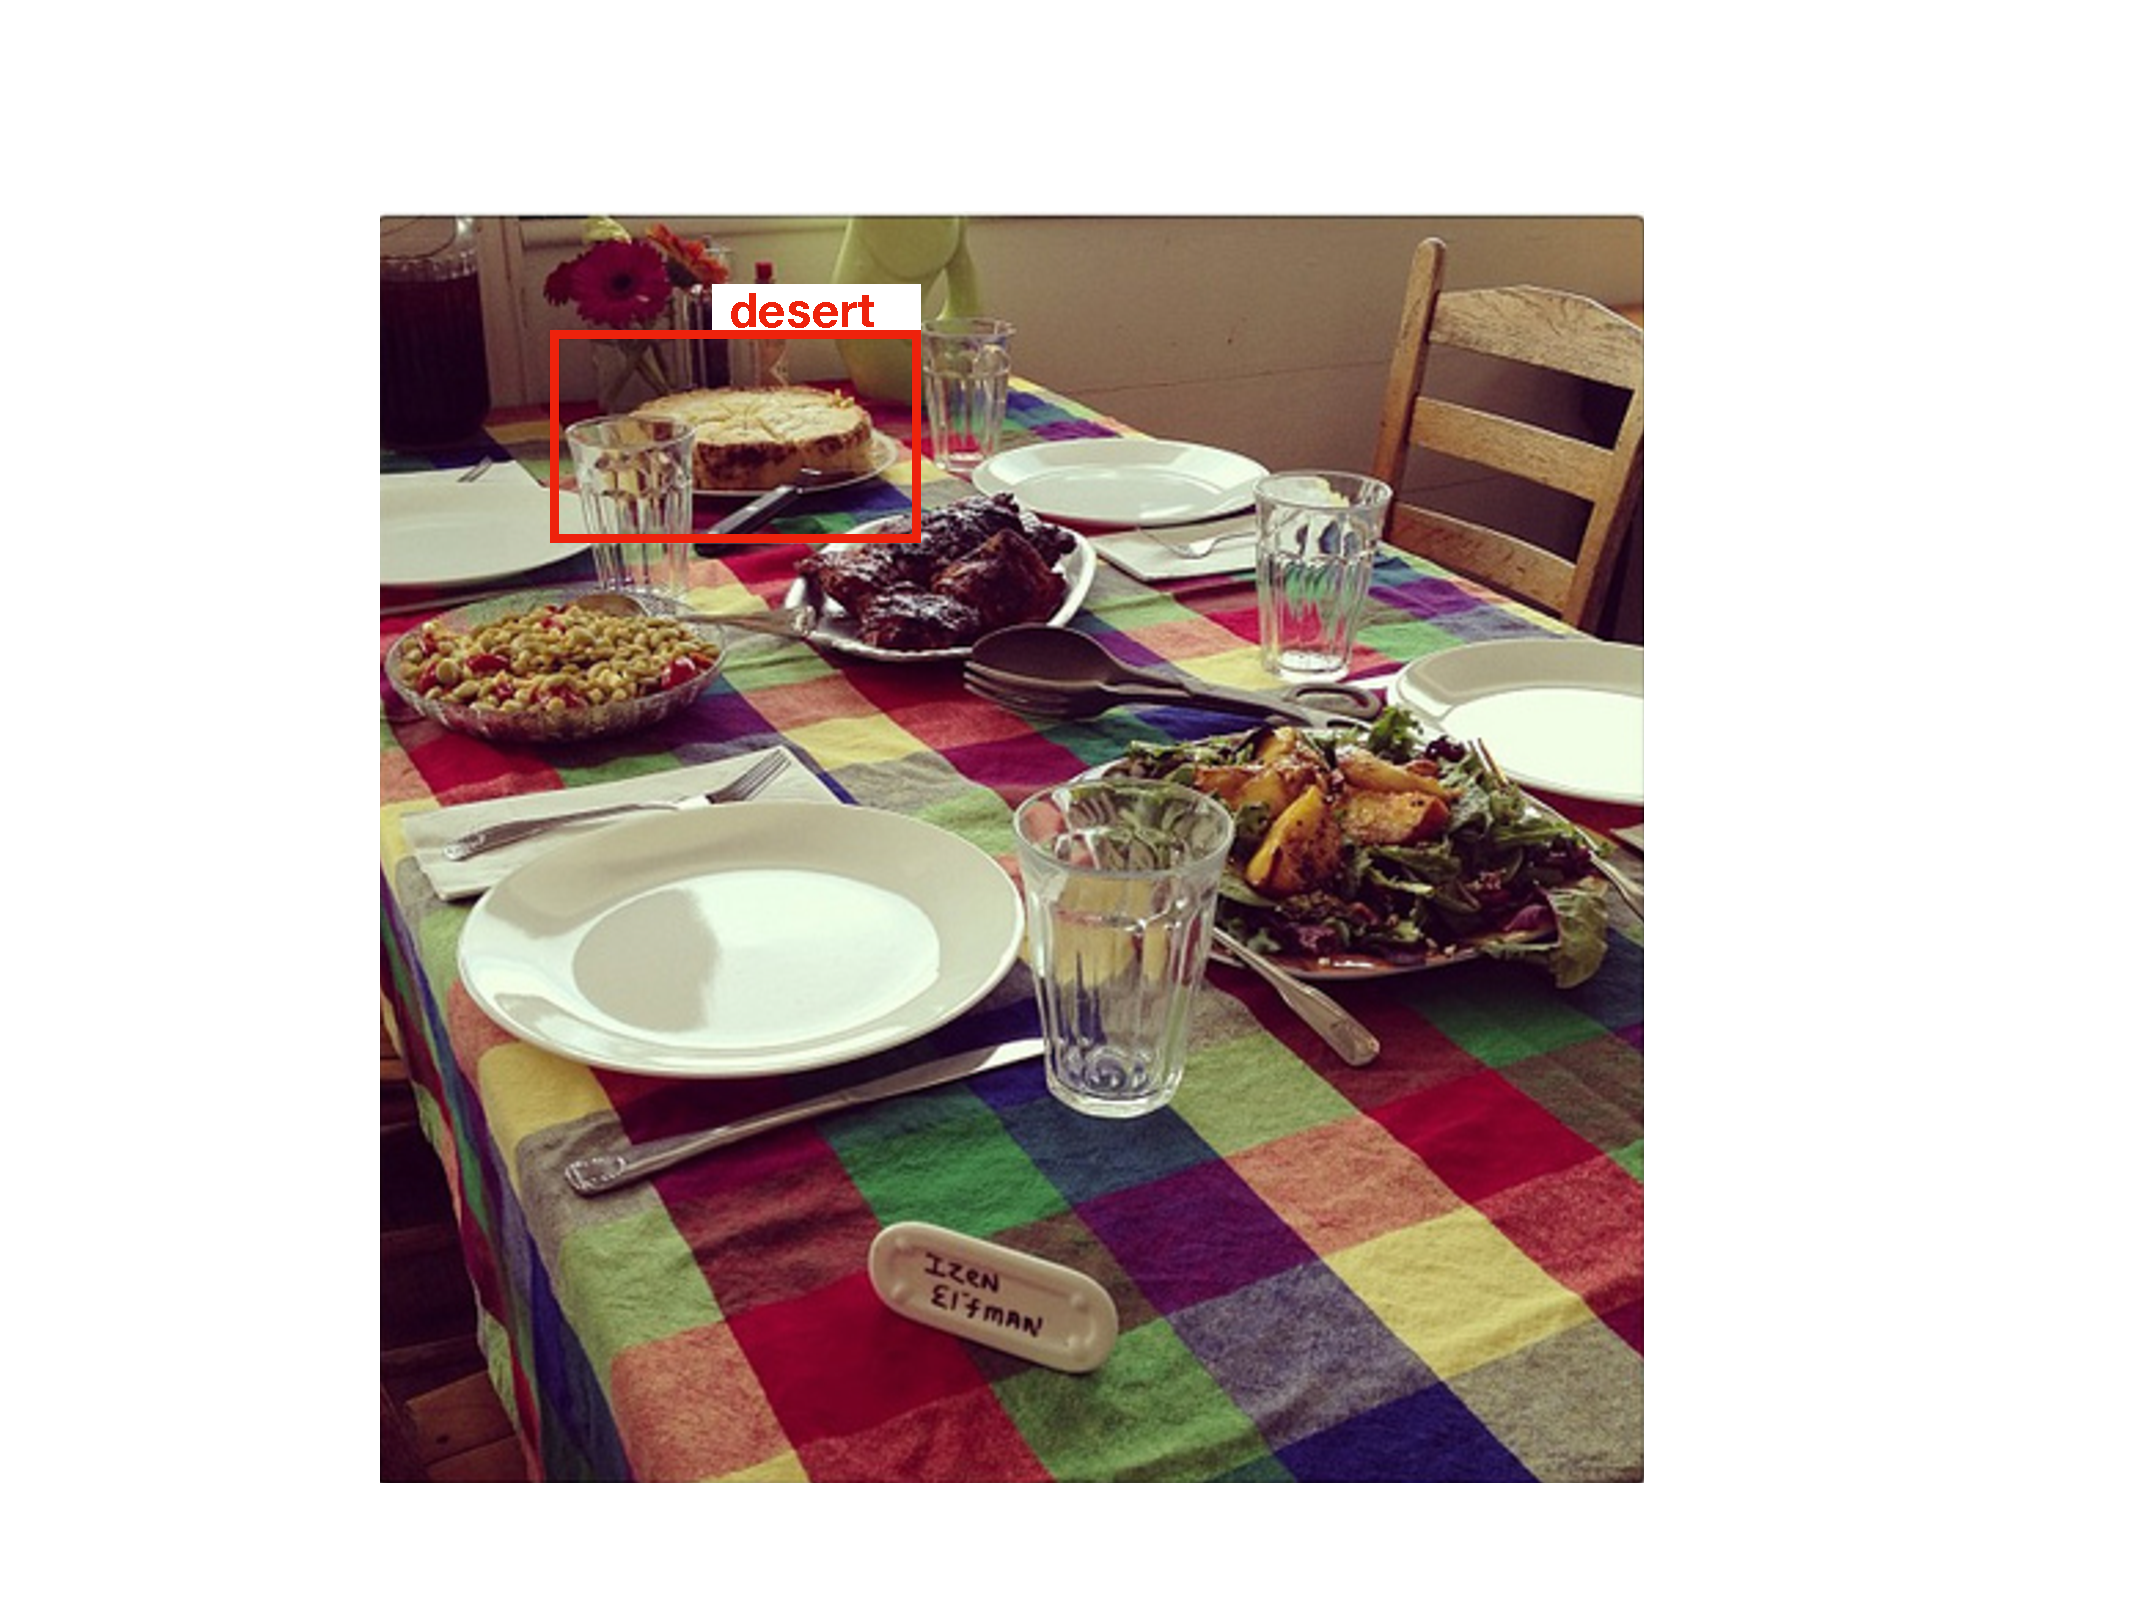
\includegraphics[height=3cm]{Figures/cheesecak2.pdf}
\caption{Two objects of the same type of cake, with different names in VisualGenome}
\label{fig:cake}
\end{center}
\end{figure}


Given the abundance of concepts available in language, the act of \textit{naming} a visual object is not just a labeling of visible properties, it amounts to selecting a name from a complex network of concepts and competing lexical alternatives.
Hence, research on cognition and language production has relied on object naming as a basic paradigm for investigating the processes that underly formation and organization of concepts in the human mind  \cite{rosch1976basic} \sz{cite more here}, though mostly using idealized, graphical objects from specific domains (plants, animals) as visual stimuli.
Complementary to that, research in computer vision has (successfully) focused on automatically recognizing \textit{real-world} objects in images or videos, but using simplified categorization schemes where each object is assigned a single correct label or name, cf.\ \cite{googlenet}. %Here, powerful models have been developed recently that classify visual objects in real-world images into thousands of different (mutually exclusive) categories \newcite{googlenet}.

In NLP, to date, research on object naming is relatively scarce despite the fact that
 there has been a recent explosion of interest in various, and even complex, language \& vision tasks ranging from image captioning \cite{fangetal:2015,devlin:imcaqui,Bernardietal:automatic} to e.g.\ visual dialogue \cite{das2017visual,vries2017guesswhat}. Massive data collections for applications in language \& vision (L\&V) are nowadays available and, in principle, these should also constitute an excellent, large-scale test beds for assessing  theories such as, e.g.\ , the claim that objects have a preferred entry-level when being named  \cite{rosch1976basic}.
%In this paper, we argue that a lot of research in this area would benefit from a deeper and more systematic understanding of the semantic and taxonomic processes in object naming, which is a core phenomenon in virtually every vision \& language task.
%At the same time, we argue that existing resources in L\&V constitute an excellent, large-scale test bed for assessing traditional claims and theories such as, e.g.\ the existence of so-called entry-level categories  \cite{rosch1976basic}.

The goal of this paper is to extend Visual Genome  \cite{krishna2016visualgenome}, a well-known, large-scale resource in language \& vision research, in a way that it can serve as a broad empirical basis for systematic and linguistically motivated investigations into object naming. 
We argue that object naming is an interesting, core phenomenon in itself as it occurs in virtually every L\&V task, but our approach can also support more systematic analysis of broader tasks, such as e.g.\ modeling referring expressions.

Even though VisualGenome is one of the most exhaustively annotated resources to date, providing dense object annotations and descriptions in real-world images, it suffers from two important shortcomings if one is interested in linguistic analysis of object naming:  
First, it only provides a single, manually annotated object description (including a single name) per object which makes it impossible to assess how representative the annotated naming choices are, e.g.\ whether speakers tend to generally prefer \refexp{cheesecake} for the highlighted object in Figure \ref{fig:cake}.
Second, it does not provide consistent taxonomic information on objects and their categories, as names have been automatically linked to WordNet synsets. 
This makes it difficult to assess how naming depends on the taxonomic properties of the object, e.g.\  that both objects in Figure \ref{fig:cake} are instances of \cat{cheesecake}, but one is named \refexp{cheesecake} and the other one is named \refexp{desert}. It is important to note here that this shortcomings exist for basically all large-scale resources currently used in L \&V research (see Section 2 below).

In this work, we address these two shortcomings and present a crowdsourcing-based and light-weight experimental set-up for eliciting representative and taxonomically consistent (\sz{more complete?}) naming data. We compare our collected data against names annotated in Visual Genome, and calculate various measures assessing agreement, naming preferences etc.

The main idea is to elicit names in (i) in a standard naming task (phase 0) where participants simply give the most straightforward name to an object they can immediately think of, and then in (ii) a taboo-like naming task where frequent names collected initially are blocked and participants have to provide alternative names. We show that this cheap, two-stage approach gives us taxonomically rich data that allows us to study object naming empirically, without adopting costly annotation procedures involving complex hierarchical object annotation schemes.


\section{Related Work}
\label{sec:related}

\paragraph{Cognition: Concepts and categorization}

 Seminal work on concepts by Rosch suggests that object names typically exhibit a preferred level of specificity called the \textbf{entry-level}. This typically corresponds to an intermediate level of specificity, i.e., \textbf{basic level} (e.g, \refexp{bird}, \refexp{car}) \cite{rosch1976basic}, as opposed to more generic (i.e., \textbf{super-level}; e.g., \refexp{animal}, \refexp{vehicle}) or specific categories (i.e., \textbf{sub-level}; e.g., \refexp{sparrow}, \refexp{convertible}). However, less prototypical members of basic-level categories tend to be instead identified with sub-level categories (e.g., a \cat{penguin} is typically called a \refexp{penguin} and not a \refexp{bird}) \cite{jolicoeur1984pictures}. 
%This out-of-context preference towards a certain taxonomic level is often referred to as \textbf{lexical availability}. 
While the traditional notion of entry-level categories suggests that objects tend to be named by a \refexp{single} preferred concept, research on pragmatics has found that speakers are flexible in  
%with respect to the chose level of specificity. 
their choice of the level of specificity. 
Scenarios where multiple objects (of the same category) are present induce a pressure for generating names which uniquely identify the target \cite{olson1970language}, such that sub-level names can be systematically elicited in these cases %\cite{rohde2012communicating} \cite{graf2016animal}. 
\cite{rohde2012communicating}\cite{graf2016animal}.

\paragraph{Vision: Object Recognition}

State-of-the-art computer vision systems are able to classify images into thousands of different categories (e.g.\  \newcite{googlenet}). These object recognition systems are now widely used in vision \& language research.
Nevertheless, the way the treat object recognition is conceptually very simple (if not to say, naive):  standard object classification schemes are inherently ``flat'', and treat object labels as mutually exclusive \cite{deng2014large}, ignoring all kinds of linguistic relations between these labels and ignoring the fact that an object can easily be an instance of several categories.


\paragraph{Vision \& language: Naming and Referring}

\newcite{Ordonez:2016} have studied the problem of deriving appropriate object names, or so-called entry-level
 categories, from the output of an object recognizer. Their approach focusses on linking abstract object categories in ImageNet to actual words via translation procedures that e.g. involve corpus frequencies. 
 \newcite{zarriess-schlangen:2017} learn a model of object naming on a corpus of referring expressions paired with objects in real-world images, but focus on combining visual and distributional information and on zero-shot learning.
 Thus, object naming is an important task for referring expression generation, though most research in this area has focussed on content and attribute selection \cite{Kazemzadeh2014,gkatzia:2015,zarrieschlang:easy-pre,Maoetal:cocorefexp}.

\paragraph{Existing resources and their shortcomings}
Moreover, existing resources in L\&V hardly provide any consistent taxonomic information on objects and their categories, e.g. object labels are typically quite general as in Flickr30k \cite{plummer2015flickr30kentities} (e.g.,~\cat{people, animals, bodyparts, clothing}) or taxonomically heterogeneous as in MS COCO \cite{mscoco} (e.g.,~\cat{people, baseball glove, bird}).





\section{Data Collection}
\label{sec:task}

describe the YouNameIt task here

\subsection{Materials} describe sampling of images, category selection

\subsection{Procedure} describe the crowdsourcing set-up and the task

\subsection{Data} give an overview of the collected data


\section{Analysis}

\subsection{Agreement, basic-level and entry-level names}

analyse data mainly from Phase 0

\begin{itemize}
\item  to what extent do people agree when their task is to give the most straightforward name they can think of to a visual object?
\item is the level of agreement the same for all categories?
\item how specific are the most familiar names? link names to WordNet, show that WordNet might not be ideal to assess specificity
\item how does agreement evolve in the later rounds of the game? (when people have to avoid taboo names), does agreement increase as the set of names becomes more narrow, or  does agreement decrease as people do creative, clever, unexpected things?
\item assess how representative name annotations in Visual Genome are, when compared to our names
\end{itemize}

\subsection{Cases of disagreement}

when and why do people give different names to the same object? this will probably happen in phase 0, and even more so in the later round \sz{this is what I expect}

\begin{itemize}
\item  analyse naming disagreement using WordNet, how do names for the same object relate to each other according to WordNet?
\item can we identify instances of cross-classification? so objects that are systematically part of several classes (e.g. cake/dessert)
\item we might need to do some manual annotation here and try to carefully describe the phenomena
\end{itemize}

\subsection{Taxonomic relations}

can we elicit natural sub-ordinate, super-ordinate concepts?

\section{Model}

\subsection{Model 1}
Train a simple naming model (classifiers) on original VisualGenome names. Test it on our data. How well does the model predict the most familiar name and the set of available names?

\subsection{Model 2}
Train a simple naming model (classifiers) on our data, maybe combined with VisualGenome data. How well does it work?

\subsection{Model 3}

can we model taxonomic/conceptual knowledge more directly? induce a taxonomy? or a multi-modal space for objects + names?

\section{Conclusion}

We have presented a systematic, large-scale study on object naming with real-world images and crowdsourced data.

\bibliography{naming}
\bibliographystyle{acl_natbib}





\end{document}

